\chapter{Project}\label{ch:project}

This chapter is devoted to the description of the general architectures, 
and specific algorithms.


\section{Logical architecture}

The logical architecture is composed by the following component:
\begin{itemize}
    \item \textbf{Web Service} a node of a peer-to-peer layer that 
        provides environment primitives to the car processes (list of adjacent cars) and, 
        at the same time, can send queries to the DB component and exposes an API for the 
        clients.
    \item \textbf{Client} a simple web page used to monitoring the simulation state; 
        uses the web service APIs to render a graphic interface that must 
        be constantly syncronized.
    \item \textbf{Car} a process that is the abstraction/simulation of a real car; 
        \begin{itemize}
            \item it can become a leader in order to schedule the crossing order for the next turn
            \item it must check the health state of the other adjacent cars 
                (calls the tow truck in case of failure)
            \item it can see environment details calling a web service 
            \item it have to syncronize its local timing using Berkeley algorith
        \end{itemize}
    \item \textbf{Distributed DBMS}, an instance of Mnesia DBMS distributed 
        on each container in order increase redundancy and robustness. 
    \item \textbf{Docker Container} wraps one or more car and/or web service instances 
        and is designed to be interconnected with all others containers 
    \end{itemize}


\section{Protocols and algorithms}

Following the \textit{divide et impera} philosophy now we are going to split the problem 
into some subproblems and solve them. 
We also provide a simplified sequence of UML (sequence) diagrams in order to 
describe the workflow/communication patterns.

\subsection{Starvation/deadlock and order method}

Ideally a car that reaches first the queue must pass before other 
incoming cars (\textbf{FIFO}).\\

We have to \textbf{avoid starvation} (ie. when a car waits infinite time cause the opposite queue 
has infinite lenght and it never has the priority) and \textbf{deadlock} (cars aren't able to 
reach the agreement). 


\subsection{Solution}

In order to avoid \textbf{starvation} in a first stage cars syncronize themselves 
(for the syncronization process we follow the \textbf{Berkeley algorithm})
in terms of local timinig and in a second stage there will be a \textbf{leader election} 
and the leader decides the crossing order. Using this method we also avoid 
the possibility of a \textbf{deadlock} as long as the leader is running.\\

In a certain instant the elected leader is the first car that has reached the bridge; 
once the current leader cross the bridge there is a new election of the car on the other 
side of the bridge (if one is present).\\


\section{Syncronization problem}

Every car has a \textbf{local timing} that can \textbf{drifts} out from the 
global timing. 

\subsection{Solution}

So we need to syncronize the incoming cars using the \textbf{Berkeley algorithm}.\\

A new incoming car calls the \textit{environment:get$\_$adjacent$\_$cars(p)} 
method in order to get the name of the adjacent cars. \\

The new car $c$ sends a message to the nearest car $n$ in order to get the current time 
(we assume that $n$ was already syncronized). 
With this information $c$ is concious of the RTT and its local drift from the global time. \\

So basically the global timing is the timing of the first leader (or the average time 
of the first block of incoming cars).\\

If some new unsyncronized cars appear in block the syncronization process takes into 
consideration the average RTT (according to the Berkeley algorithm). 


\section{Agreement}

The current leader identifies the block of cars that will cross the bridge and notifies
this decision.  

\subsection{Solution}

Before crossing the bridge, the leader propagates a message to 
the first n cars behind him (where n is the capacity of the bridge) telling them to cross the bridge
and the identity of the first car B on the other side. Each car, who 
receives the message, checks if its arrival time is less then B's: if so, the car can 
cross the bridge too, otherwise waits for its turn.\\
The leader will always be elected by himself. Suppose the car A, that is not leader
 and that has not the permission to cross, arrives at the last position
before the bridge. At that point A checks if there are any cars in front of her:
\begin{itemize}
\item if there is a car whose arrival time is greater then A's and is on the opposite side
then A is the new leader;
\item if there isn't any cars then A is the new leader 
\end{itemize}

\begin{center}
    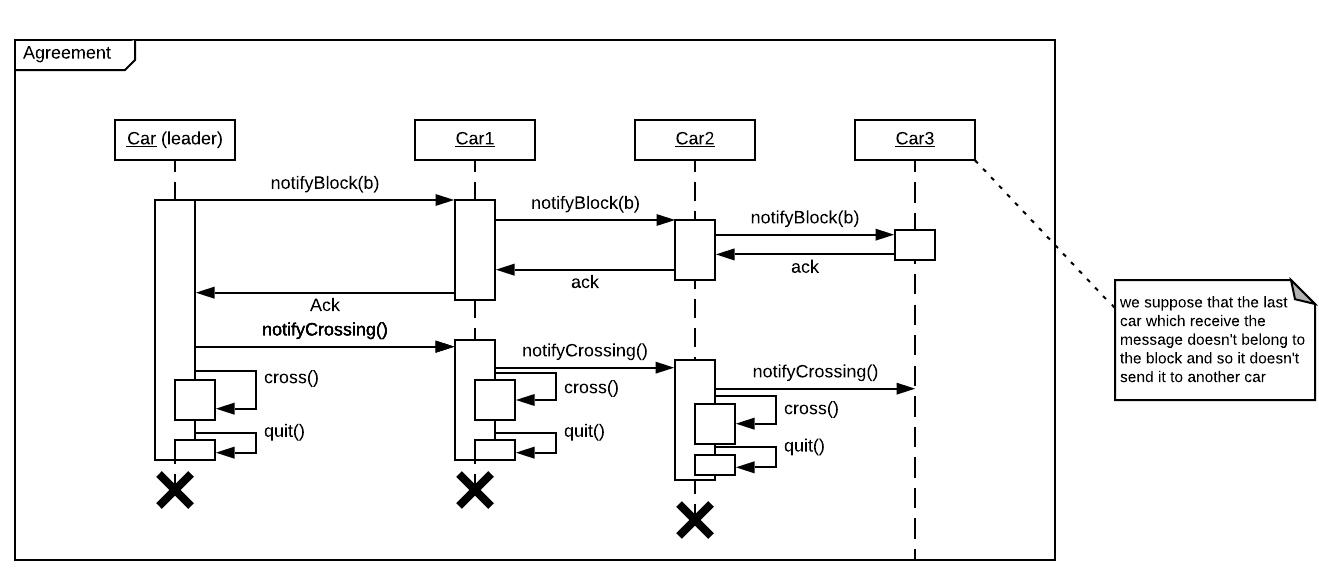
\includegraphics[scale=0.6]{assets/ds2019_3.png}
\end{center}


\section{Failures}

In case of failure, of both engine and communication system,
 another car has to call a \textbf{tow truck} for help. If only the engine has crashed then the car
 itself can call the \textbf{tow truck}.

\subsection{Solution}

Each car recursively checks if other reachable cars are safe; if a check message
hasn't any response within a certain \textbf{timeout} (depends on the RTT) it is assumed 
that the receiver has a failure (and so the tow truck will be call). Then the car have to wait to be removed 
and then notify the first car behind that she has been removed after the tow truck timeout.
The car has also to tell the name of the car in front of her so that the rear one can communicate with the next one. \\
Every time something like that happens, the remaining cars must update their adjacent lists.

\begin{center}
    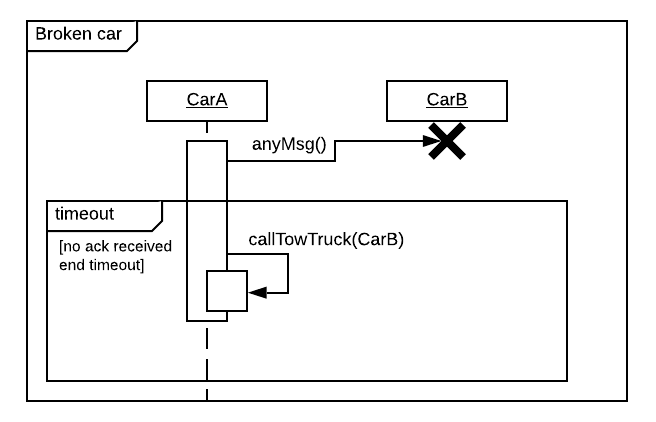
\includegraphics[scale=0.9]{assets/ds2019_4.png}
\end{center}


\section{MIM attack}

The system must withstand a MIM attack.


\subsection{Solution}

Each message will be encrypted (HTTPS).


\section{Scalability}

The system must \textbf{scale wrt. the load} 
(the number of cars and clients can scale arbitrary).


\subsection{Solution}

Assume that the available machines are defined in an arbitrary 
way in the initialization phase; on each machine some docker containers 
will be raised and foreach one of those an arbitrary number of web services and 
car processes will be spawned.\\


[Bonus requirement, not necessary]
We will design an embedded load balancer in order to avoid the web services overload 
(considering the number of calls).

\begin{center}
    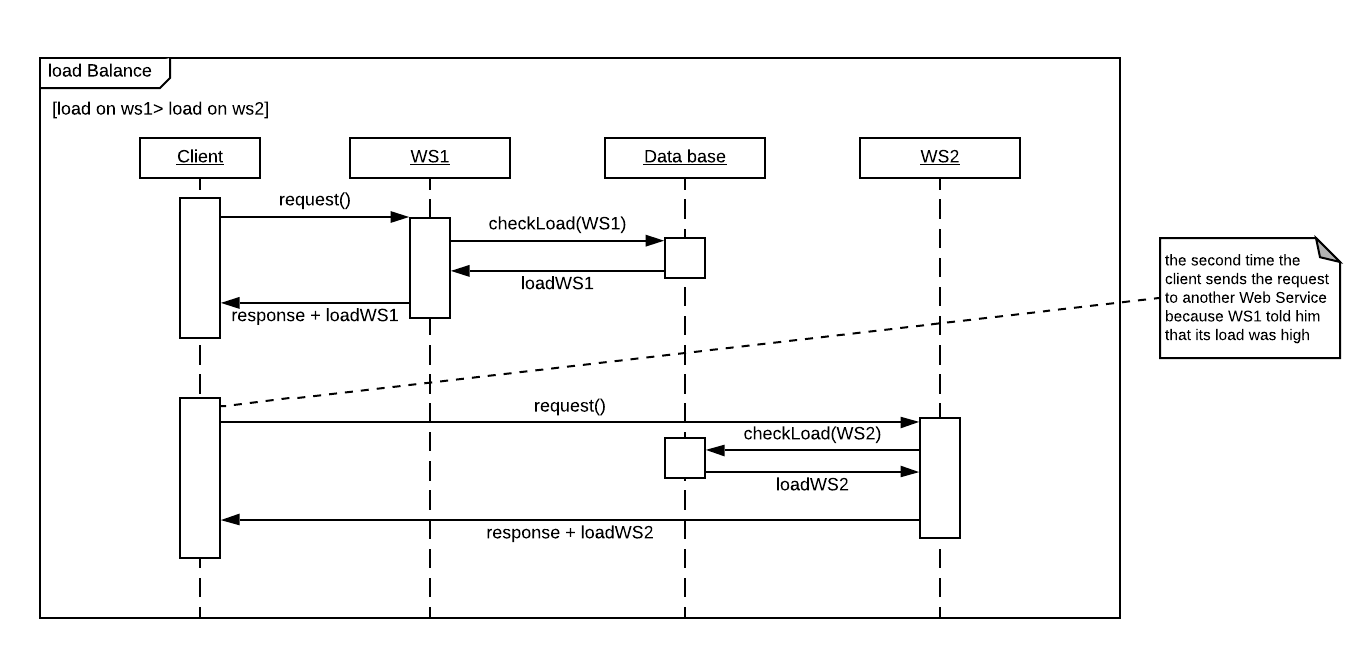
\includegraphics[scale=0.6]{assets/ds2019_2.png}
\end{center}


\section{SPOF}

The system must be resilient wrt. failures (even multiple failures);
so basically the architecture must be deeply \textbf{distributed} 
and \textbf{decentralized} (avoid any SPOF). 


\subsection{Solution}

The scalability requirement imposes that every macro-component must be scalable 
so the architecture provides some \textbf{peer-to-peer layers} 
(web services layer, cars layer).
The only SPOF in this context can be the \textit{environment} component 
(which is embedded into the web services) that allows for a new spawned car to 
start a message exchange with the adjacent cars. 
A possible solution can be using a \textbf{distributed DBMS} like Mnesia~\cite{1} in order to keep 
track of the queue state.

\begin{center}
    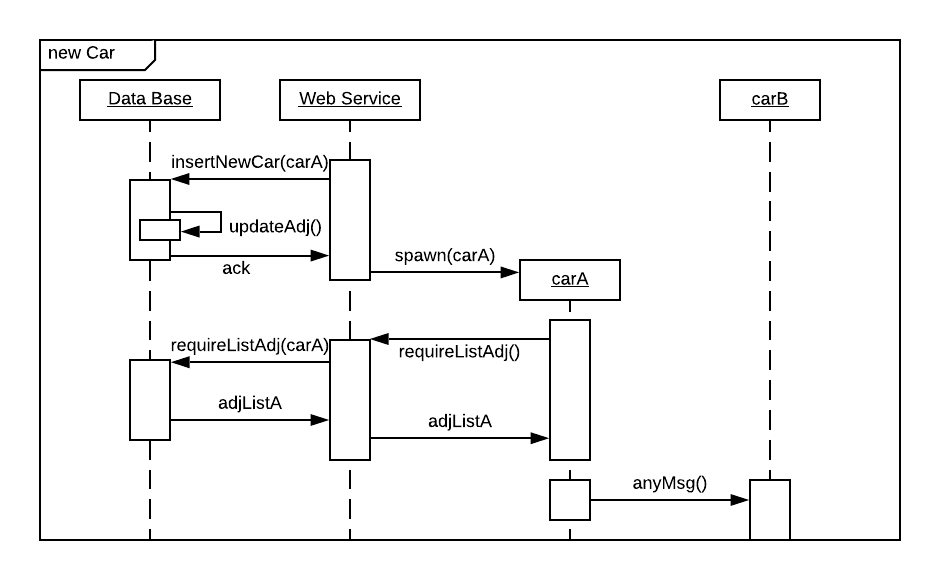
\includegraphics[scale=0.8]{assets/ds2019_1.png}
\end{center}

\begin{center}
    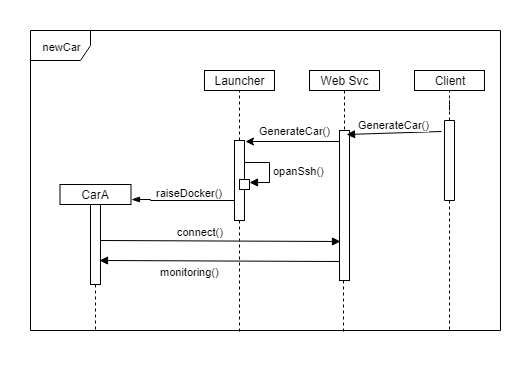
\includegraphics[scale=0.6]{assets/newCarclient.png}
\end{center}

\begin{center}
    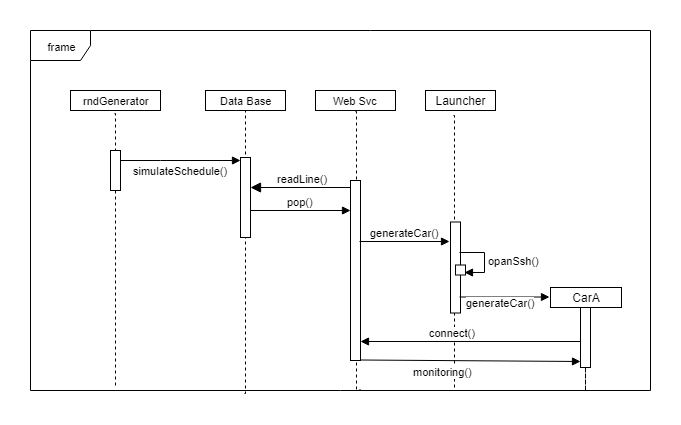
\includegraphics[scale=0.6]{assets/newCarRnd.png}
\end{center}


\subsection{Algorithms}

We have used the Berkeley algorithm in order to syncronize new spawned car processes.

\begin{center}
    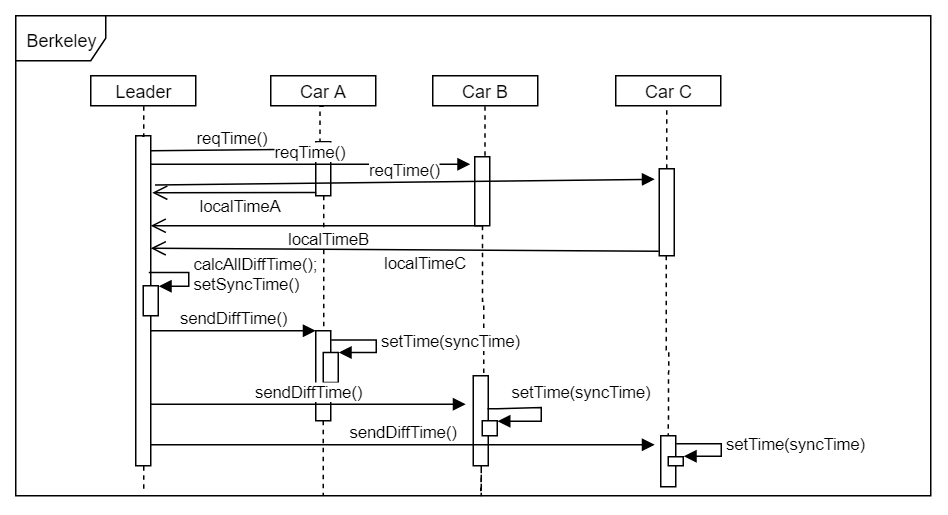
\includegraphics[scale=0.6, width=\linewidth]{assets/berkeley.png}
\end{center}

\section{Physical architecture and deployment}

The deployment and start up consists in the following steps:
\begin{enumerate}
    \item Get the ssh credentials of each computer involved in the simulation
    \item Execute a launcher bash script that will open an ssh tunnel with each computer and 
        raise the Docker Containers with an arbitrary number of web services 
    \item A random generator or a test procedure inserts into the DB a simulation schedule
        (the web service p2p layer starts automatically the simulation)
    \item With a web browser any client can connect to the web service API and monitoring 
        the simulation state   
\end{enumerate}

The code required for the simulation is taken directly from the project repository hosted on 
GitHub~\cite{2}.


\section{Development plan}

The proposed architecture is a \textbf{P2P} architecture flanked by a 
\textbf{client-server} architecture (\textbf{three-tier architecture}: client, web service and DBMS).
